%%%% Paramétrage du TD %%%%
\def\xxactivite{\ifcolle Colle \else Application 3 \fi  \ifprof -- Corrigé \else \fi} % \normalsize \vspace{-.4cm}
\def\xxauteur{\textsl{Xavier Pessoles}}

\def\xxnumchapitre{Chapitre 3 \vspace{.2cm}}
\def\xxchapitre{\hspace{.12cm} Méthodologie : détermination des équations de mouvement}
\def\xxpartie{Modéliser le comportement des systèmes mécaniques dans le but d'établir une loi de comportement ou de déterminer des actions mécaniques en utilisant le PFD}



\def\xxtitreexo{Chaîne ouverte -- Centrifugeuse géotechnique \ifnormal $\star$ \else \fi \ifdifficile $\star\star$ \else \fi \iftdifficile $\star\star\star$ \else \fi }

\def\xxsourceexo{\hspace{.2cm} \footnotesize{Pôle Chateaubriand -- Joliot Curie}}


\def\xxcompetences{%
\vspace{-.5cm}
\textsl{%
\textbf{Savoirs et compétences :}
\begin{itemize}[label=\ding{112},font=\color{ocre}] 
%\item \textit{Mod2.C16} : torseur cinétique
%\item \textit{Mod2.C17} : torseur dynamique
%\item \textit{Mod2.C17.SF1} : déterminer le torseur dynamique d’un solide, ou d’un ensemble de solides, par rapport à un autre solide
%\item \textit{Mod2.C15} : matrice d'inertie
\item \textit{Res1.C2} : principe fondamental de la dynamique
\item \textit{Res1.C1.SF1} : proposer une démarche permettant la détermination de la loi de mouvement
%\item \textit{Res1.C2.SF1} : proposer une méthode permettant la détermination d’une inconnue de liaison
\end{itemize}
}}
\def\xxfigures{
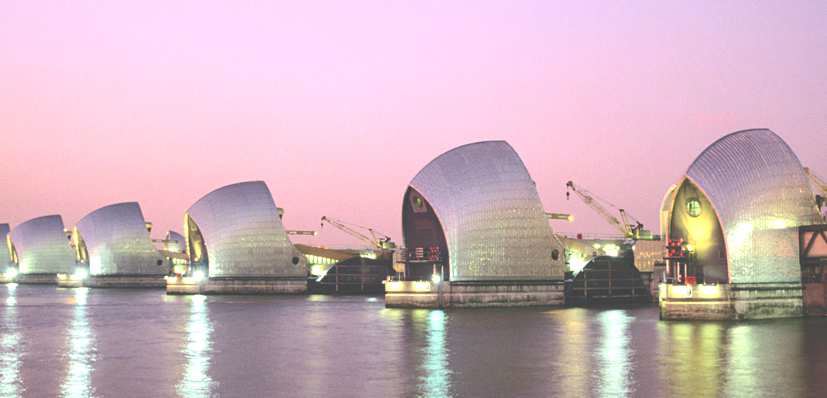
\includegraphics[width=.35\linewidth]{fig_00}
}%figues de la page de garde


\input{\repRel/Style/pagegarde_TD}
\setcounter{numques}{0}

\setlength{\columnseprule}{.1pt}

\pagestyle{fancy}
\thispagestyle{plain}

\ifprof
\vspace{4.8cm}
\else
\vspace{4.8cm}
\fi

\def\columnseprulecolor{\color{ocre}}
\setlength{\columnseprule}{0.4pt} 

%%%%%%%%%%%%%%%%%%%%%%%

\setcounter{exo}{0}





\ifprof
\else
\begin{multicols}{2}

\subsection*{Présentation}
La géotechnique correspond aux activités liées aux applications de la mécanique des sols, de la mécanique des roches et de la
géologie. À partir d'essais en laboratoire et in situ, la géotechnique fournit aux constructeurs de bâtiments et d'ouvrages les
données indispensables pour le génie civil en ce qui concerne leur stabilité en fonction des sols. Aujourd'hui la modélisation
physique d'ouvrage géotechnique en centrifugeuse est une approche expérimentale répandue. La centrifugation des modèles
réduits permet de reproduire des états de contraintes dans les matériaux semblables à ceux régnant dans l'ouvrage grandeur
nature. Le laboratoire central des Ponts et Chaussées (LCPC) de Nantes possède une centrifugeuse géotechnique dont les
principales caractéristiques sont données ci-après :
\begin{itemize}
\item distance de l'axe à la plate-forme nacelle : \SI{5,5}{m};
\item longueur du bras : \SI{6,8}{m};
\item accélération maximale : \SI{200}{g};
\item temps de montée à \SI{200}{g} : \SI{360}{s}.
\end{itemize}

On propose le modèle cinématique suivant :
\begin{center}
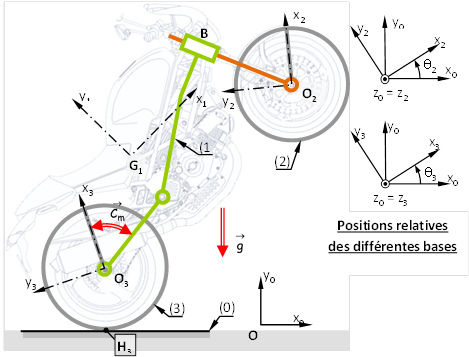
\includegraphics[width=\linewidth]{fig_01}
\end{center}

Soit $\mathcal{R}=\repere{O}{x}{y}{z}$ un repère galiléen lié au bâti 0 de la centrifugeuse. L'axe $\axe{O}{z}$ est dirigé suivant la verticale descendante. 
On désigne par $\vect{g}=g\vect{z}$ le vecteur accélération de la pesanteur.

Le bras 1 est en liaison pivot sans frottement d’axe $\axe{O}{z}$ avec le bâti 0. Soit $\mathcal{R}_1=\repere{O}{x_1}{y_1}{z}$ un repère lié au bras 1. On pose $\alpha=\angl{x}{x_1}$, avec $\alpha=\omega t$, où $\omega$ est une constante positive. 

La nacelle 2 est en liaison pivot sans frottement d’axe $\axe{A}{y_1}$ avec le bras 1 , telle que $\vect{OA}=a\vect{x_1}$ ($a$ est une constante positive). Soit $\mathcal{R}_2=\repere{A}{x_2}{y_1}{z_2}$ un repère lié à la nacelle 2. On pose $\beta=\angl{z}{z_2}$. 

On note :
\begin{itemize}
\item bras 1 : moment d’inertie $I$ par rapport à l’axe $\axe{O}{z}$;
\item nacelle 2 : centre d’inertie $G$ , tel que $\vect{AG}=b\vect{z_2}$ ($b$ est une constante positive), masse $m$, 
matrice d’inertie $\inertie{A}{2}=\matinertie{A}{B}{C}{0}{0}{0}{\mathcal{B}_2}$. 
\end{itemize}
Un moteur, fixé sur la bâti 0, exerce sur le bras 1 une action mécanique représentée par le couple $C_m\vect{z}$.
Le bras 1 tourne à la vitesse constante $\omega$ par rapport au bâti 0.

\begin{obj}
Déterminer les équations du mouvement de la centrifugeuse, ainsi que le couple moteur à fournir au cours du
mouvement.
\end{obj}

\question{Préciser le théorème à utiliser permettant de déterminer l’équation de mouvement de la nacelle 2 par rapport au
bras 1. Déterminer cette équation.}
\ifprof
\begin{corrige}
\end{corrige}
\else
\fi

\question{Préciser le théorème à utiliser permettant de déterminer le couple moteur. Déterminer son expression.}
\ifprof
\begin{corrige}
\end{corrige}
\else
\fi

On suppose que la nacelle 2 est en équilibre relatif par rapport au bras 1, et que $mba> > A \simeq C$.

\question{Déterminer les expressions de l’angle $\beta$ et du couple moteur $C_m$ ?}
\ifprof
\begin{corrige}
\end{corrige}
\else
\fi


%\vspace{1cm}
%\paragraph*{Éléments de correction}
%\footnotesize
%\begin{enumerate}
%\item $-mgb\sin \beta = B\ddot{\beta}+\omega^2 \cos\beta \left[\sin\beta\left(C-A\right)-mba\right]$.
%\item $C_m=2\omega\dot{\beta}\cos\beta  \left[\sin\beta\left(A-C\right)+mba\right]$.
%\item $\beta=\arctan\left( \dfrac{\omega^2 a}{g}\right)$ et $C_m=0$.
%\end{enumerate}

\end{multicols}
\fi

\ifprof

\begin{center}
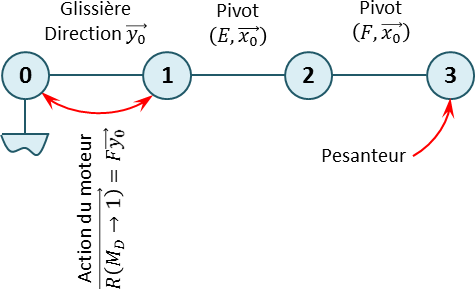
\includegraphics[width=.8\linewidth]{cor_01}
\end{center}

\begin{center}
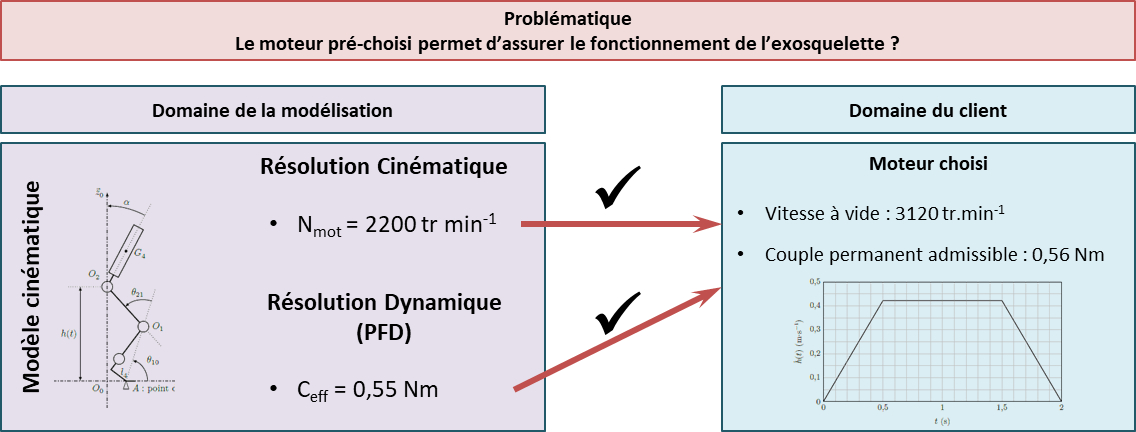
\includegraphics[width=\linewidth]{cor_02}
\end{center}

\begin{center}
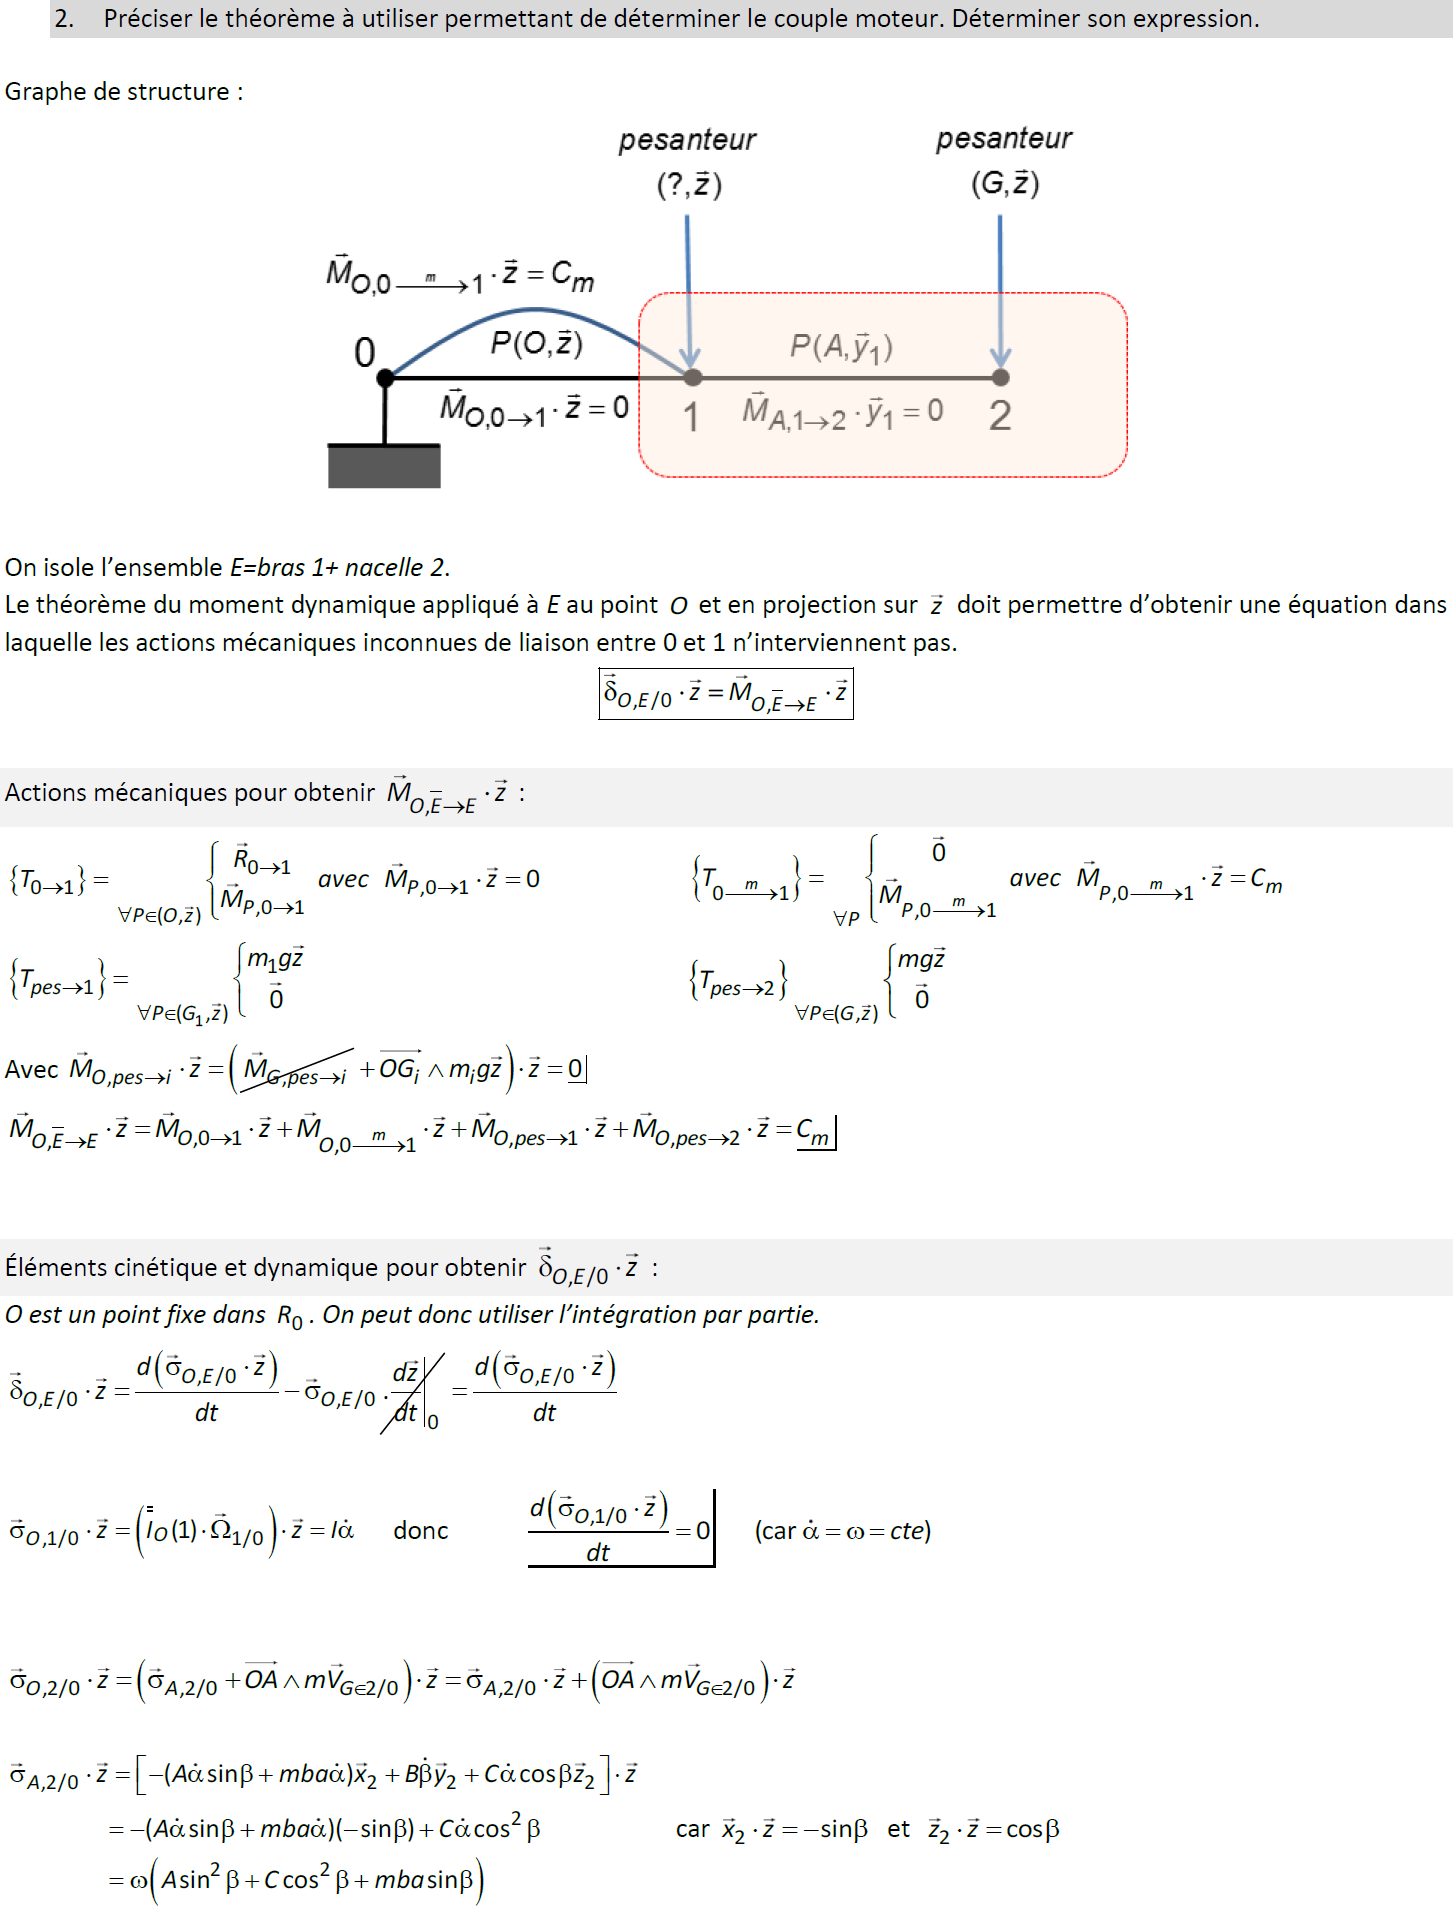
\includegraphics[width=\linewidth]{cor_03}
\end{center}

\begin{center}
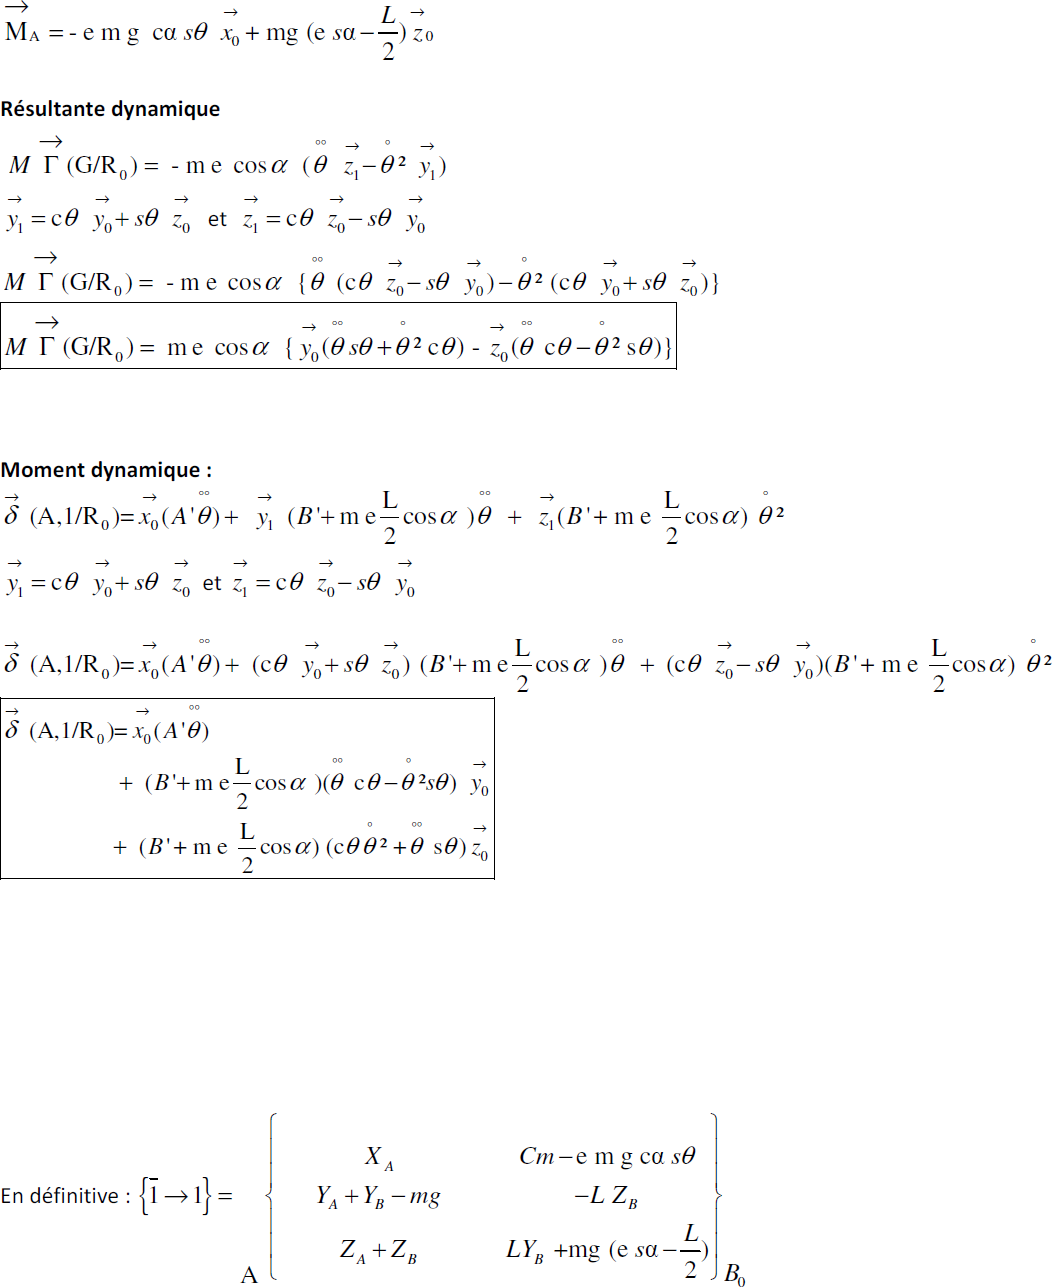
\includegraphics[width=\linewidth]{cor_04}
\end{center}
\else
\fi